\begin{problem}{\kcpcpapercuttitle}
    {표준 입력}{표준 출력}
    {\kcpcpapercuttime\,초}{\kcpcpapercutmemory\,MB}{}{\kcpcpapercutscore}
    고려대학교의 대표아싸 중 한명인 인구는 혼자놀기의 달인이다. 인구는 가로와 세로의 길이가 무한대인 종이를 무한대로 가지고 있다. 인구가 가진 종이는 너무 커서 필요한 만큼 잘라 쓴다. 인구는 이 특별한 종이를 자를 수 있는 유일한 도구인 직선칼을 가지고 있는데, 이 칼을 써서 종이를 자르면 자른 선분을 무한히 연장한 직선으로 종이가 잘린다. 인구는 다각형 모양으로 종이를 자르려고 하는데, 다음과 같은 과정을 거친다.
    
    \begin{itemize}
        \item 아직 자르지 않은 변 하나를 고른다.
        \item 그 변을 포함하는 직선을 자른다. 더 이상 자를 변이 없을 경우 종료한다.
        \item 종이를 그대로 놔둔 채로 1번으로 돌아간다.
    \end{itemize}
    위의 과정을 거쳐 자를 경우 다각형의 일부에 속하는 종이 조각과 다각형에 속하지 않는 종이 조각으로 나눌 수 있는데, 인구는 문득 그 숫자가 궁금해졌다. 그 두 수를 각각 구하시오.
    
    단, 직선칼은 이미 나누어진 종이라도 직선상에 있으면 끝까지 자른다. 또 각 변을 연장해서 생기는 직선들과 이들이 만나 생기는 교점들에 대해, 어떤 세 점도 일직선상에 있지 않으며 어떤 세 직선도 한점에서 만나지 않음이 보장된다. 또 임의의 두 교점 사이의 거리는 $ 10^{-6} $ 이상임이 보장된다.
    
    \InputFile
    첫 번째 줄에 인구가 가지고 놀 다각형의 변의 개수 $ N $ 이 주어진다. $ (3 \leq N \leq 1,000) $
    
    두 번째 줄부터 $ N $개의 줄에 걸쳐 다각형의 꼭짓점의 좌표가 시계 방향으로 주어지며, 각 줄마다 두 정수 $ x_i, y_i $ 가 공백으로 구분하여 주어진다. $ (-10^6 \leq x_i,\ y_i \leq 10^6) $
    
    입력으로 주어진 다각형의 서로 다른 두 변은 교차하지 않음이 보장된다.
    \OutputFile
    첫 번째 줄에 다각형의 일부에 속하는 종이조각의 개수를 출력한다.
    
    두 번째 줄에 다각형의 일부에 속하지 않는 종이조각의 개수를 출력한다.
    
    \SubtaskWithScore{\kcpcpapercutsmallscore}
    주어지는 다각형의 모든 변은 $ x $축 또는 $ y $축에 평행하다.
    
    \SubtaskWithScore{\kcpcpapercutlargescore}
    문제 입력에서 주어진 조건 외에 추가적인 조건이 없다.

    \Examples
    
    \begin{example}
        \exmp{
            3
            0 0
            0 2
            2 0
        }{%
            1
            6 
        }%
        \exmp{
            4
            4 0
            0 0
            0 4
            1 1
        }{%
            3
            8
        }%              
    \end{example}
    
    \Explanation
    첫 번째 예제의 모습은 다음과 같다.
    \begin{figure}[h]
        \centering
        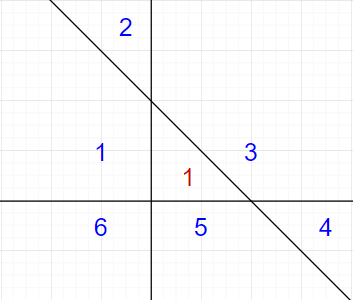
\includegraphics[width=0.3\textwidth]{./problems/papercut-ex1.png}
    \end{figure}
    
    두 번째 예제의 모습은 다음과 같다.
    \begin{figure}[h]
        \centering
        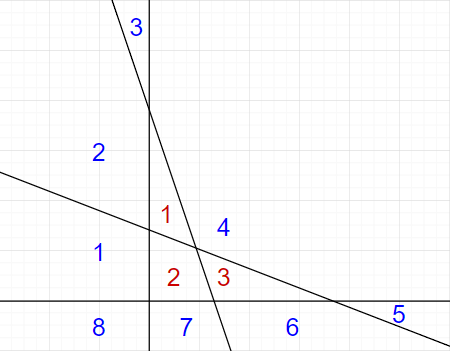
\includegraphics[width=0.3\textwidth]{./problems/papercut-ex2.png}
    \end{figure}
\end{problem}

